\documentclass[compress]{beamer}
\usetheme{Warsaw}
\useoutertheme{split}

%%%%%%%%%%%%%%%%%%%%%%%%%%%%%%%%%%%%%%%%%%%%%%%%%%%%%%%%%%%%%%%
% Improvement on the default split theme : added line numbers %
%%%%%%%%%%%%%%%%%%%%%%%%%%%%%%%%%%%%%%%%%%%%%%%%%%%%%%%%%%%%%%%
\defbeamertemplate*{footline}{mysplit theme}
{%
  \leavevmode%
  \hbox{\begin{beamercolorbox}[wd=.5\paperwidth,ht=2.5ex,dp=1.125ex,leftskip=.3cm plus1fill,rightskip=.3cm]{author in head/foot}%
    \usebeamerfont{author in head/foot}\insertshortauthor
  \end{beamercolorbox}%
  \begin{beamercolorbox}[wd=.4\paperwidth,ht=2.5ex,dp=1.125ex,leftskip=.3cm,rightskip=.3cm plus1fil]{title in head/foot}%
    \usebeamerfont{title in head/foot}\insertshorttitle
  \end{beamercolorbox}}%
    \begin{beamercolorbox}[wd=.1\paperwidth,ht=2.5ex,dp=1.125ex,leftskip=.2cm plus1fill,rightskip=.3cm]{date in head/foot}
      \usebeamerfont{date in head/foot} \insertframenumber{} / \inserttotalframenumber 
    \end{beamercolorbox}
  \vskip0pt%
}

%%%%%%%%%%%%
% packages %
%%%%%%%%%%%%

\usepackage{minted}
\newminted{cpp}{gobble=4,linenos}
\newminted[shell]{shell-session}{gobble=4}
\newminted[makefile]{shell-session}{gobble=4}

\usepackage{pgf}
\usepackage{pgffor}
\usepackage{tikz}
\usetikzlibrary{arrows,automata,snakes,shapes}

\usepackage[framemethod=TikZ]{mdframed}
\mdfdefinestyle{simplebox}{roundcorner=4pt,linewidth=0,backgroundcolor=blue!50!black,fontcolor=white}

\usepackage{multicol}

%%%%%%%%%%%%%%%%%%%
% useful commands %
%%%%%%%%%%%%%%%%%%%
\newcommand{\cpp}{C$^{++}$} 

%%%%%%%%%%%%%%%%%%%%%%%%%%%%%%%
% easy class diagrams in tikz %
%%%%%%%%%%%%%%%%%%%%%%%%%%%%%%%

\newcommand\classbox[3][]{
  \draw[thick] node (#2) [#1]
       [rectangle,rounded corners,draw] {
    \begin{tabular}{l}
      \multicolumn{1}{c}{#2} \\
      #3
    \end{tabular}
  };
}

%%%%%%%%%%%%%%%%%%%%%%%%%%%%%%%%%%%%%%
% easy memory stack diagrams in tikz %
%%%%%%%%%%%%%%%%%%%%%%%%%%%%%%%%%%%%%%

\newcounter{memorystackindex}

\pgfkeys{
  memorystack/.is family,
  memorystack,
  size x/.initial=4cm,
  size y/.initial=.5cm,
  word size/.initial=4,
  nb blocks/.initial=8,
  base address/.initial=12351,
  color/.initial=black
}

\makeatletter

\newcommand\memorystackset[1]{\pgfkeys{memorystack,#1}}
\newcommand\memorystack[1][]{
  \memorystackset{#1,
    size x/.get=\stacksizex,
    size y/.get=\stacksizey,
    word size/.get=\stackwordsize,
    nb blocks/.get=\stacknbblocks,
    base address/.get=\stackbaseaddr,
    color/.get=\stackcolor
  }
  \draw[thick,\stackcolor,text=white] node (title)
        at (\stacksizex/2, \stacknbblocks*\stacksizey+.5cm)
        [rectangle,rounded corners,fill=blue!50!black] {Memory layout};
  \setcounter{memorystackindex}{1}
  \draw[thick,\stackcolor] (0,0) rectangle (\stacksizex,\stacknbblocks*\stacksizey);
  \pgfmathsetmacro{\nbbars}{\stacknbblocks-1}
  \pgfmathtruncatemacro\nbbarstrunc{\nbbars}
  \ifnum\nbbarstrunc>0
    \foreach \n in {1,...,\nbbars} {
      \draw[\stackcolor!70] (0,\n*\stacksizey) -- +(\stacksizex,0);
    }
  \fi
  \foreach \n in {1,...,\stacknbblocks} {
    \foreach \p in {1,...,\stackwordsize} {
      \draw node (stack\n-\p)
            at (\stacksizex/\stackwordsize*\p-\stacksizex/\stackwordsize/2,\n*\stacksizey-\stacksizey/2)
            [rectangle,minimum width=\stacksizex,minimum height=\stacksizey] {};
    }
    \pgfmathparse{\n*\stackwordsize+\stackbaseaddr}
    \pgfmathdectoBase\hexversion{\pgfmathresult}{16}
    \draw node at (\stacksizex,\n*\stacksizey-\stacksizey/2) [right=2pt]
          {0x\hexversion};
  }
  \pgfmathsetmacro{\nbseps}{\stackwordsize-1}
  \pgfmathtruncatemacro\nbsepstrunc{\nbseps}
  \ifnum\nbsepstrunc>0
    \foreach \n in {1,...,\nbseps} {
      \draw[\stackcolor!10] (\stacksizex/\stackwordsize*\n,0) -- +(0,\stacknbblocks*\stacksizey);
    }
  \fi
}

\newcommand\memorypushvalue[3]{
  \draw node at (stack#1-#2) {#3};
}

\newcounter{localcount}
\newcommand\memorypush[1]{
  \memorystackset{
    word size/.get=\stackwordsize,
    nb blocks/.get=\stacknbblocks
  }
  \count@=0
  \setcounter{localcount}{1}
  \@for\v:=#1\do{
    \ifnum\count@<\stackwordsize
      \advance\count@ 1
      \memorypushvalue{\arabic{memorystackindex}}{\arabic{localcount}}{\v}
    \fi
    \addtocounter{localcount}{1}
  }  
  \addtocounter{memorystackindex}{1}
}

\newcommand\memorypushpointer[2][]{
  \memorystackset{
    word size/.get=\stackwordsize,
    base address/.get=\stackbaseaddr
  }
  \pgfmathparse{#2*\stackwordsize+\stackbaseaddr}
  \pgfmathdectoBase\hexaddress{\pgfmathresult}{16}
  \memorypushvalue{\arabic{memorystackindex}}{1}{#1 0x\hexaddress}
  \draw[\stackcolor!80,->] (stack\arabic{memorystackindex}-1.west) .. controls +(left:1) and +(left:1) .. (stack#2-1.west);
  \addtocounter{memorystackindex}{1}
}

\newcommand\memorystruct[3]{
  \memorystackset{
    size y/.get=\stacksizey
  }
  \draw[snake=brace,thick] (-2pt,#1*\stacksizey-\stacksizey) -- (-2pt,#2*\stacksizey)
    node [midway, above, sloped] {#3};
}

\newcommand\memorygoto[1]{
  \setcounter{memorystackindex}{#1}
}
\makeatother

%%%%%%%%%%%%%%%%%%
% Document setup %
%%%%%%%%%%%%%%%%%%

\title{\cpp course}
\author[S. Ponce]{S\'ebastien Ponce  \texttt{sebastien.ponce@cern.ch}}
\institute{CERN}
\date{ESIPAP Feb 24th 2014}
\pgfdeclareimage[height=0.5cm]{cernlogo}{CERN-logo.jpg}
\logo{\pgfuseimage{cernlogo}}

\AtBeginSection[] {
  \begin{frame}<beamer>
    \frametitle{TOC Section}
    \setcounter{tocdepth}{2}
    \tableofcontents[sectionstyle=show/shaded,subsectionstyle=show/show/hide]
  \end{frame}
}

%%%%%%%%%%%%%%
% The slides %
%%%%%%%%%%%%%%

\begin{document}

\begin{frame}
  \titlepage
\end{frame}

\begin{frame}
  \frametitle{Foreword}
  \begin{block}{What this course is not}
    \begin{itemize}
    \item It is not for complete beginners
    \item It is not for experts
    \item This is not complete at all
    \end{itemize}
  \end{block}
  \begin{block}{What it should be}
    \begin{itemize}
    \item Adaptative
    \item Interactive
    \item Useful
    \end{itemize}
  \end{block}
\end{frame}

\begin{frame}
  \frametitle{Outline}
  \tableofcontents[sectionstyle=show,subsectionstyle=hide]
\end{frame}

\section[Introduction]{History and goals}
%\section[Intro]{History and goals}

\subsection[Hist]{History}

\begin{frame}
  \frametitle{C/\cpp origins}
  \begin{minipage}{0.4\linewidth}
    \tikzstyle{old}=[ellipse,draw=black,fill=orange!30,thick,inner sep=2pt]
    \tikzstyle{new}=[rectangle,draw=black,fill=green!50,thick,inner sep=2pt]
    \tikzstyle{direct}=[<-,semithick]
    \tikzstyle{transverse}=[<-,dotted,semithick]
    \begin{tikzpicture}[->, node distance=.75cm, font=\tiny, scale=0.9, every node/.style={scale=0.9}]
      \node[old] (Simula)      {Simula};
      \node[left of=Simula,node distance=1.5cm] {1967};
      \node[old] (BCPL) [right of=Simula, node distance=2cm] {BCPL};
      \node[old] (B) [below of=BCPL] {B}
      edge[transverse] (BCPL);
      \node[old] (KandRC) [below of=B] {K and R C}
      edge[transverse] (B);
      \node[left of=KandRC,node distance=3.5cm] {1978};
      \node[old] (ClassicC) [below of=KandRC] {Classic C}
      edge[direct] (KandRC);
      \node[old] (CwithClasses) [below of=Simula,node distance=3cm] {C with Classes}
      edge[transverse] (Simula)
      edge[transverse] (BCPL)
      edge[direct] (ClassicC);
      \node[left of=CwithClasses,node distance=1.5cm] {1980};
      \node[old] (EarlyC++) [below of=CwithClasses] {Early \cpp}
      edge[direct] (CwithClasses);
      \node[left of=EarlyC++,node distance=1.5cm] {1985};
      \node[old] (C89) [below of=ClassicC,node distance=2.25cm] {C89}
      edge[direct] (ClassicC)
      edge[transverse] (CwithClasses);
      \node[old] (ARMC++) [below of=EarlyC++] {ARM \cpp}
      edge[direct] (EarlyC++)
      edge[transverse] (C89);
      \node[left of=ARMC++,node distance=1.5cm] {1989};
      \node[old] (C++98) [below of=ARMC++] {\cpp98}
      edge[direct] (ARMC++)
      edge[transverse] (C89);
      \node[old] (C99) [below of=C89] {C99}
      edge[direct] (C89)
      edge[transverse] (ARMC++);
      \node[left of=C++98,node distance=1.5cm] {1998};
      \node[new] (C++11) [below of=C++98] {\cpp11}
      edge[direct] (C++98)
      edge[transverse] (C99);
      \node[left of=C++11,node distance=1.5cm] {2011};
      \node[new] (C11) [below of=C99] {C11}
      edge[direct] (C99)
      edge[transverse] (C++98);
      \node[new] (C18) [below of=C11,node distance=1.8cm] {C18}
      edge[direct] (C11);
      \node[new] (C++14) [below of=C++11] {\cpp14}
      edge[direct] (C++11);
      \node[left of=C++14,node distance=1.5cm] {2014};
      \node[new] (C++17) [below of=C++14] {\cpp17}
      edge[direct] (C++14);
      \node[left of=C++17,node distance=1.5cm] {2017};
      \node[new] (C++20) [below of=C++17] {\cpp20}
      edge[direct] (C++17);
      \node[left of=C++20,node distance=1.5cm] {2020};
    \end{tikzpicture}
  \end{minipage}
  \begin{minipage}{0.57\linewidth}
    \begin{tabular}{cc}
      \includegraphics[height=2.5cm]{ritchie.jpeg} & \includegraphics[height=2.5cm]{BjarneStroustrup.jpg} \\[-1ex]
      \tiny{C inventor} & \tiny{\cpp inventor} \\[-1ex]
      \scriptsize{Dennis M. Ritchie} & \scriptsize{Bjarne Stroustrup} \\
    \end{tabular}
    \begin{itemize}
      {\footnotesize
      \item Both C and \cpp are born in Bell Labs
      \item \cpp {\it almost} embeds C
      \item C and \cpp are still under development
      \item We will discuss all \cpp specs
      \item Each slide will be marked with first spec introducting the feature
      }
    \end{itemize}
  \end{minipage}
\end{frame}

\begin{frame}
  \frametitle{\cpp11, \cpp14, \cpp17, \cpp20...}
  \begin{block}{status}
    \begin{itemize}
    \item A new \cpp specification every 3 years
      \begin{itemize}
      \item \cpp20 is ready, supposed to be official in May
      \end{itemize}
    \item Bringing each time a lot of goodies
    \end{itemize}
  \end{block}
  \pause
  \begin{block}{How to use \cpp XX features}
    \begin{multicols}{2}
      \begin{itemize}
      \item Use a compatible compiler
      \item add -std=c++xx to compilation flags
      \item e.g. -std=c++17
      \end{itemize}
      \vfill
      \columnbreak
      \begin{table}[h!]
        \begin{center}
          \begin{tabular}{c|c|c}
            \textbf{\cpp} & \textbf{gcc} & \textbf{clang}\\
            \hline
            11 & $\geq$4.8 & $\geq$3.3\\
            14 & $\geq$4.9 & $\geq$3.4\\
            17 & $\geq$7.3 & $\geq$5\\
            20 & $>$10  & $>$10 \\
          \end{tabular}
          \caption{Minimum versions of gcc and clang for a given \cpp version}
        \end{center}
      \end{table}
    \end{multicols}
  \end{block}
\end{frame}

\subsection[Use]{Why we use it ?}

\begin{frame}
  \frametitle{Why is \cpp our language of choice ?}
  \begin{block}{Adapted to large projects}
    \begin{itemize}
    \item strongly typed
    \item object oriented
    \item widely used (and taught)
    \item many available libraries
    \end{itemize}
  \end{block}
  \pause
  \begin{block}{Fast}
    \begin{itemize}
    \item compiled (unlike Java or C\#)
    \item allows to go close to hardware when needed
    \end{itemize}
  \end{block}
  \pause
  \begin{alertblock}{What we get}
    \begin{itemize}
    \item the most powerful language
    \item the most complicated one
    \item the most error prone ?
    \end{itemize}
  \end{alertblock}
\end{frame}


\section[Basics]{Langage basics (C and \cpp)}
%\section[base]{Language basics}

\subsection[Core]{Core syntax and types}

\begin{frame}[fragile]
  \frametitlecpp[98]{Hello World}
  \begin{cppcode}
    #include <iostream>

    // This is a function
    void print(int i) {
      std::cout << "Hello, world " << i << std::endl;
    }

    int main(int argc, char** argv) {
      int n = 3;
      for (int i = 0; i < n; i++) {
        print(i);
      }
      return 0;
    }
  \end{cppcode}
\end{frame}

\begin{frame}[fragile]
  \frametitlecpp[98]{Comments}
  \begin{cppcode}
    // simple comment until end of line
    int i;

    /* multiline comment
     * in case we need to say more
     */
    double /* or something in between */ d;

    /**
     * Best choice : doxygen compatible comments
     * \brief checks whether i is odd
     * \param i input
     * \return true if i is odd, otherwise false
     * \see https://www.doxygen.nl/manual/docblocks.html
     */
    bool isOdd(int i);
  \end{cppcode}
\end{frame}

\begin{frame}[fragile]
  \frametitlecpp[98]{Basic types(1)}
  \begin{cppcode}
    bool b = true;            // boolean, true or false

    char c = 'a';             // min 8 bit integer
                              // may be signed or not
                              // can store an ASCII character
    signed char c = 4;        // min 8 bit signed integer
    unsigned char c = 4;      // min 8 bit unsigned integer

    char* s = "a C string";   // array of chars ended by \0
    string t = "a C++ string";// class provided by the STL

    short int s = -444;       // min 16 bit signed integer
    unsigned short s = 444;   // min 16 bit unsigned integer
    short s = -444;           // int is optional
  \end{cppcode}
\end{frame}
\begin{frame}[fragile]
  \frametitlecpp[98]{Basic types(2)}
  \begin{cppcode}
    int i = -123456;          // min 16, usually 32 bit
    unsigned int i = 1234567; // min 16, usually 32 bit

    long l = 0L               // min 32 bit
    unsigned long l = 0UL;    // min 32 bit

    long long ll = 0LL;          // min 64 bit
    unsigned long long l = 0ULL; // min 64 bit

    float f = 1.23f;          // 32 (23+8+1) bit float
    double d = 1.23E34;       // 64 (52+11+1) bit float
    long double ld = 1.23E34L // min 64 bit float
  \end{cppcode}
\end{frame}

\begin{frame}[fragile]
  \frametitlecpp[98]{Portable numeric types}
  \alert{Requires inclusion of a specific header}
  \begin{cppcode}
    #include <cstdint>

    int8_t c = -3;     // 8 bit signed integer
    uint8_t c = 4;     // 8 bit unsigned integer

    int16_t s = -444;  // 16 bit signed integer
    uint16_t s = 444;  // 16 bit unsigned integer

    int32_t s = -0674; // 32 bit signed integer
    uint32_t s = 0674; // 32 bit unsigned integer

    int64_t s = -0x1bc;// 64 bit signed integer
    uint64_t s = 0x1bc;// 64 bit unsigned int
    \end{cppcode}
\end{frame}

\begin{frame}[fragile]
  \frametitlecpp[98]{Useful aliases}
    \alert{Requires inclusion of headers}
  \begin{cppcode}
    #include <cstddef> // and many other headers

    size_t s = sizeof(int); // unsigned integer
                            // can hold any variable's size

    #include <cstdint>

    ptrdiff_t c = &s - &s;  // signed integer, can hold any
                            // diff between two pointers

    // int, which can hold any pointer value:
    intptr_t i = reinterpret_cast<intptr_t>(&s);   // signed
    uintptr_t i = reinterpret_cast<uintptr_t>(&s); // unsigned
    \end{cppcode}
\end{frame}

\subsection[Ptr]{Arrays and Pointers}

\begin{frame}[fragile]
  \frametitlecpp[98]{Static arrays}
  \begin{cppcode}
    int ai[4] = {1,2,3,4};
    int ai[] = {1,2,3,4};  // identical

    char ac[3] = {'a','b','c'};   // char array
    char ac[4] = "abc";           // valid C string
    char ac[4] = {'a','b','c',0}; // same valid string

    int i = ai[2];  // i = 3
    char c = ac[8]; // at best garbage, may segfault
    int i = ai[4];  // also garbage !
  \end{cppcode}
\end{frame}

\Scontents*[store-cmd=code_arrays]{
int i = 4;
int *pi = &i;
int j = *pi + 1;

int ai[] = {1,2,3};
int *pai = ai;
int *paj = pai + 1;
int k = *paj + 1;

// not compiling
int *pak = k;

// seg fault !
int *pak = (int*)k;
int l = *pak;
}
\begin{frame}[fragile]
  \frametitlecpp[98]{Pointers}
  \begin{multicols}{2}
  \begin{overprint}[\columnwidth]
    \onslide<1> \highlightCppCode{}{code_arrays}
    \onslide<2> \highlightCppCode{1}{code_arrays}
    \onslide<3> \highlightCppCode{2}{code_arrays}
    \onslide<4> \highlightCppCode{3}{code_arrays}
    \onslide<5> \highlightCppCode{5}{code_arrays}
    \onslide<6> \highlightCppCode{6}{code_arrays}
    \onslide<7> \highlightCppCode{7}{code_arrays}
    \onslide<8> \highlightCppCode{8}{code_arrays}
    \onslide<9> \highlightCppCode{11}{code_arrays}
  \end{overprint}
  \columnbreak
    \onslide<2->{
      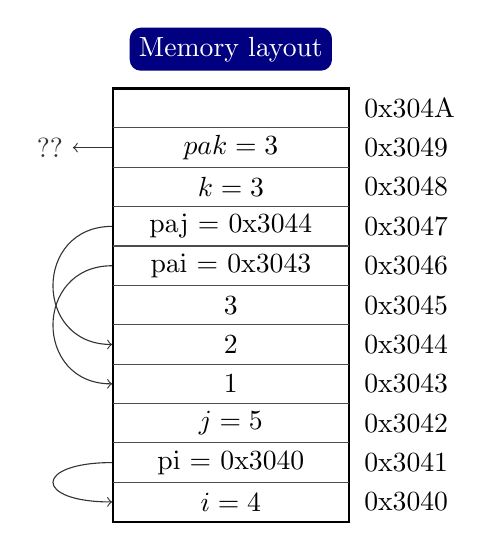
\begin{tikzpicture}
        \memorystack[size x=3cm,word size=1,nb blocks=11]
        \onslide<2-> {\memorypush{$i = 4$}}
        \onslide<3-> {\memorypushpointer[pi =]{1}}
        \onslide<4-> {\memorypush{$j = 5$}}
        \onslide<5-> {\memorypush{$1$}}
        \onslide<5-> {\memorypush{$2$}}
        \onslide<5-> {\memorypush{$3$}}
        \onslide<6-> {\memorypushpointer[pai =]{4}}
        \onslide<7-> {\memorypushpointer[paj =]{5}}
        \onslide<8-> {\memorypush{$k = 3$}}
        \onslide<9-> {\memorypush{$pak = 3$}}
        \onslide<9-> {\draw[\stackcolor!80,->] (stack10-1.west) -- +(-0.5cm,0)
          node [anchor=east] {??};}
      \end{tikzpicture}
    }
  \end{multicols}
\end{frame}

\begin{frame}[fragile]
  \frametitlecpp[11]{nullptr}
  \begin{block}{Finally a \cpp~NULL pointer}
    \begin{itemize}
    \item if a pointer doesn't point to anything, set it to \mintinline{cpp}{nullptr}
    \item works like 0 or NULL in standard cases
    \item triggers compilation error when mapped to integer
    \end{itemize}
  \end{block}
  \pause
  \begin{exampleblock}{Example code}
    \begin{cppcode*}{}
      void* vp = nullptr;
      int* ip = nullptr;
      int i = NULL;      // OK -> bug ?
      int i = nullptr;   // ERROR
    \end{cppcode*}
  \end{exampleblock}
\end{frame}

\begin{frame}[fragile]
  \frametitlecpp[98]{Dynamic Arrays}
  \begin{cppcode}
    #include <cstdlib>
    #include <cstring>

    int *bad;          // pointer to random address
    int *ai = nullptr; // better. Can be tested

    // allocate array of 10 ints (not initialized)
    ai = (int*) malloc(10*sizeof(int));
    // and set them to 0
    memset(ai, 0, 10*sizeof(int));

    // both in one go
    ai = (int*) calloc(10, sizeof(int));

    // release memory
    free(ai);
  \end{cppcode}
\end{frame}

\subsection[NS]{Scopes / namespaces}

\begin{frame}[fragile]
  \frametitlecpp[98]{Scope}
  \begin{block}{Definition}
    Portion of the source code where a given name is valid \\
    Typically :
    \begin{itemize}
    \item simple block of code, within \mintinline{cpp}{{}}
    \item function, class, namespace
    \item translation unit for global declarations
    \end{itemize}
  \end{block}
  \begin{exampleblock}{Example}
    \begin{cppcode*}{}
      { int a;
        { int b;
        } // end of b scope
      } // end of a scope
    \end{cppcode*}
  \end{exampleblock}
\end{frame}

\Scontents*[store-cmd=code_scopes]{
int a = 1;
{
  int b[4];
  b[0] = a;
}
// Doesn't compile:
// b[1] = a + 1;
}
\begin{frame}[fragile]
  \frametitlecpp[98]{Scope and lifetime of resources}
  \begin{block}{Resource life time}
    \begin{itemize}
      \item Resources are allocated when declared
      \item Resources are freed at the end of a scope
      \item Good practice: initialise resources when allocating!
    \end{itemize}
  \end{block}
  \begin{multicols}{2}
    \begin{overprint}[\columnwidth]
    \onslide<1>
    \highlightCppCode{1}{code_scopes}
    \onslide<2>
    \highlightCppCode{3}{code_scopes}
    \onslide<3>
    \highlightCppCode{4}{code_scopes}
    \onslide<4>
    \highlightCppCode{7}{code_scopes}
    \end{overprint}

    \columnbreak

    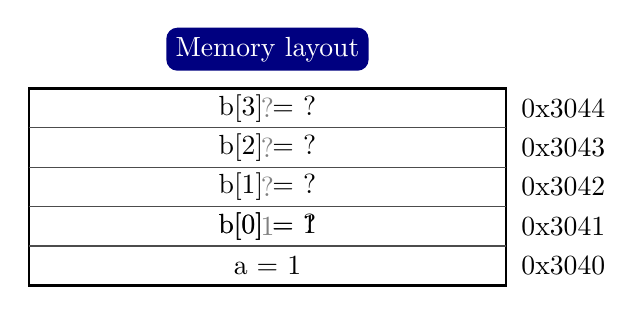
\begin{tikzpicture}
      \memorystack[word size=1, nb blocks=5, size x = 0.5\columnwidth]
      \onslide<1-> {
        \memorypush{a = 1}
      }
      \onslide<2>{
        \memorypush{b[0] = ?}
      }
      \memorygoto{2}
      \onslide<3>{
        \memorypush{b[0] = 1}
      }
      \memorygoto{3}
      \onslide<2-3>{
        \memorypush{b[1] = ?}
        \memorypush{b[2] = ?}
        \memorypush{b[3] = ?}
      }

      \memorygoto{2}
      \onslide<4>{
        \memorypush{\color{gray} 1}
        \memorypush{\color{gray} ?}
        \memorypush{\color{gray} ?}
        \memorypush{\color{gray} ?}
        }

    \end{tikzpicture}

  \end{multicols}
\end{frame}

\begin{frame}[fragile]
  \frametitlecpp[98]{Namespaces}
  \begin{itemize}
  \item Namespaces allow to segment your code to avoid name clashes
  \item They can be embedded to create hierarchies (separator is '::')
  \end{itemize}
  \begin{multicols}{2}
    \begin{cppcode*}{gobble=2}
      int a;
      namespace n {
        int a;   // no clash
      }
      namespace p {
        int a;   // no clash
        namespace inner {
          int a; // no clash
        }
      }
      int f() {
        n::a = 2;
      }
    \end{cppcode*}
    \columnbreak
    \begin{cppcode*}{gobble=2,firstnumber=14}
      namespace p {
        int f() {
          p::a = 2;
          a = 2;  //same as above
          p::inner::a = 4;
          inner::a = 4;
          n::a = 5;
        }
      }
      using namespace p::inner;
      int g() {
        a = 3; // using p::inner
      }
  \end{cppcode*}
  \end{multicols}
\end{frame}

\begin{frame}[fragile]
  \frametitlecpp[17]{Nested namespaces}
  Easier way to declare nested namespaces
  \begin{alertblock}{\cpp14}
    \begin{cppcode*}{}
      namespace A {
        namespace B {
          namespace C {
            //...
          }
        }
      }
    \end{cppcode*}
  \end{alertblock}
  \begin{exampleblock}{\cpp17}
    \begin{cppcode*}{}
      namespace A::B::C {
        //...
      }
    \end{cppcode*}
  \end{exampleblock}
\end{frame}

\begin{frame}[fragile]
  \frametitlecpp[98]{Anonymous namespaces}
  \begin{exampleblock}{A namespace without a name !}
    \begin{cppcode*}{}
      namespace {
        int localVar;
      }
    \end{cppcode*}
  \end{exampleblock}
  \begin{block}{Purpose}
    \begin{itemize}
    \item groups a number of declarations
    \item visible in the current translation unit
    \item but not reusable outside
    \item allows much better compiler optimizations and checking
      \begin{itemize}
      \item e.g. unused function warning
      \item context dependent optimizations
      \end{itemize}
    \end{itemize}
  \end{block}
  \begin{alertblock}{Deprecates static}
    \begin{cppcode*}{gobble=2}
      static int localVar; // equivalent C code
    \end{cppcode*}
  \end{alertblock}
\end{frame}

\subsection[Class/Enum]{Class and enum types}

\begin{frame}[fragile]
  \frametitlecpp[98]{struct}
  \begin{mdframed}[style=simplebox]
    \center ``members'' grouped together under one name
  \end{mdframed}
  \begin{multicols}{2}
    \begin{cppcode*}{gobble=2}
      struct Individual {
        unsigned char age;
        float weight;
      };

      Individual student;
      student.age = 25;
      student.weight = 78.5f;

      Individual teacher = {
        45, 67.0f
      };
    \end{cppcode*}
    \columnbreak
    \begin{cppcode*}{gobble=2,firstnumber=14}
      Individual *ptr = &student;
      ptr->age = 25;
      // same as: (*ptr).age = 25;
    \end{cppcode*}
    \pause
    \vfill
    \hspace{-1.5cm}
    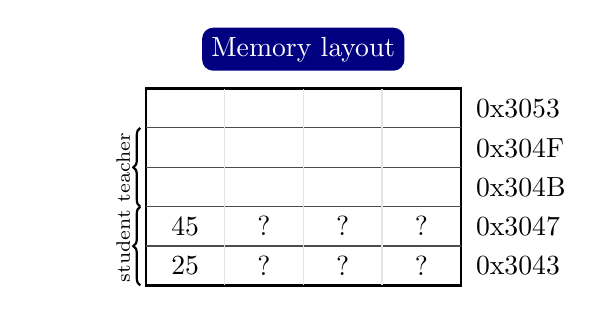
\begin{tikzpicture}
      \memorystack[nb blocks=5]
      \onslide<3-> {
        \memorypush{25,?,?,?}
        \memorypushwidevalue{78.5}
        \memorystruct{1}{2}{\scriptsize student}
      }
      \onslide<4-> {
        \memorypush{45,?,?,?}
        \memorypushwidevalue{67.0}
        \memorystruct{3}{4}{\scriptsize teacher}
      }
    \end{tikzpicture}
    \vfill \null
  \end{multicols}
\end{frame}

\begin{frame}[fragile]
  \frametitlecpp[98]{union}
  \begin{mdframed}[style=simplebox]
    \center ``members'' packed together at same memory location
  \end{mdframed}
  \begin{multicols}{2}
    \begin{cppcode*}{gobble=2}
      union Duration {
        int seconds;
        short hours;
        char days;
      };
      Duration d1, d2, d3;
      d1.seconds = 259200;
      d2.hours = 72;
      d3.days = 3;
      d1.days = 3; // d1.seconds overwritten
      int a = d1.seconds; // d1.seconds is garbage
    \end{cppcode*}
    \pause
    \columnbreak
    \null \vfill
    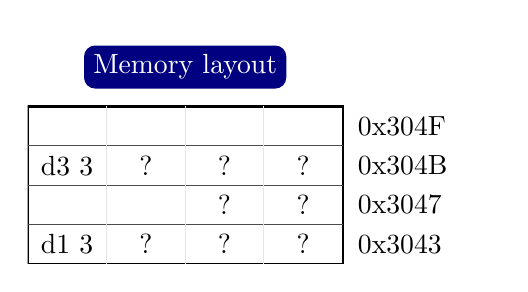
\begin{tikzpicture}
      \clip (0,0) rectangle (6cm, 3cm);
      \memorystack[word size=4,nb blocks=4]
      \visible<3-5>{\memorypushwidevalue{d1 259200}}
      \onslide<4->{\memorypushhalfvalue{d2 72}}
      \memorygoto{2}
      \onslide<4->{\memorypush{,,?,?}}
      \onslide<5->{\memorypush{d3 3,?,?,?}}
      \memorygoto{1}
      \onslide<6->{\memorypush{d1 3,?,?,?}}
    \end{tikzpicture}
    \vfill \null
  \end{multicols}
  \onslide<7->{
  \begin{alertblock}{}
    Starting with \cpp17: prefer \mintinline{cpp}{std::variant}
  \end{alertblock}
  }
\end{frame}

\begin{frame}[fragile]
  \frametitlecpp[98]{Enums}
  \begin{block}{}
    \begin{itemize}
        \item use to declare a list of related constants (enumerators)
        \item has an underlying integral type
        \item enumerator names leak into enclosing scope
    \end{itemize}
  \end{block}
  \begin{multicols}{2}
    \begin{cppcode*}{gobble=2}
      enum VehicleType {

        BIKE,  // 0
        CAR,   // 1
        BUS,   // 2
      };
      VehicleType t = CAR;
    \end{cppcode*}
    \columnbreak
    \begin{cppcode*}{gobble=2}
      enum VehicleType
        : int { // C++11
        BIKE = 3,
        CAR = 5,
        BUS = 7,
      };
      VehicleType t2 = BUS;
    \end{cppcode*}
  \end{multicols}
\end{frame}

\begin{frame}[fragile]
  \frametitlecpp[11]{Scoped enumeration, aka enum class}
  \begin{block}{Same syntax as enum, with scope}
    \begin{cppcode*}{}
      enum class VehicleType { Bus, Car };
      VehicleType t = VehicleType::Car;
    \end{cppcode*}
  \end{block}
  \pause
  \begin{exampleblock}{Only advantages}
    \begin{itemize}
    \item scopes enumerator names, avoids name clashes
    \item strong typing, no automatic conversion to int
    \end{itemize}
    \small
    \begin{cppcode*}{}
      enum VType { Bus, Car }; enum Color { Red, Blue };
      VType t = Bus;
      if (t == Red) { /* We do enter */ }
      int a = 5 * Car; // Ok, a = 5

      enum class VT { Bus, Car }; enum class Col { Red, Blue };
      VT t = VT::Bus;
      if (t == Col::Red) { /* Compiler error */ }
      int a = t * 5;       // Compiler error
    \end{cppcode*}
  \end{exampleblock}
\end{frame}

\begin{frame}[fragile]
  \frametitlecpp[98]{More sensible example}
  \begin{multicols}{2}
    \begin{cppcode*}{gobble=2}
      enum class ShapeType {
        Circle,
        Rectangle
      };

      struct Rectangle {
        float width;
        float height;
      };
    \end{cppcode*}
    \columnbreak
    \pause
    \begin{cppcode*}{gobble=2,firstnumber=10}
      struct Shape {
        ShapeType type;
        union {
          float radius;
          Rectangle rect;
        };
      };
    \end{cppcode*}
  \end{multicols}
  \pause
  \begin{multicols}{2}
    \begin{cppcode*}{gobble=2,firstnumber=17}
      Shape s;
      s.type =
        ShapeType::Circle;
      s.radius = 3.4;

    \end{cppcode*}
    \columnbreak
    \begin{cppcode*}{gobble=2,firstnumber=20}
      Shape t;
      t.type =
        Shapetype::Rectangle;
      t.rect.width = 3;
      t.rect.height = 4;
    \end{cppcode*}
  \end{multicols}
\end{frame}

\begin{frame}[fragile]
  \frametitle{typedef and using \hfill \cpp98 / \cpp11}
  Used to create type aliases
  \begin{alertblock}{\cpp98}
    \begin{cppcode*}{gobble=2}
      typedef uint64_t myint;
      myint toto = 17;
      typedef int pos[3];
    \end{cppcode*}
  \end{alertblock}
  \begin{exampleblock}{\cpp11}
    \begin{cppcode*}{gobble=2}
      using myint = uint64_t;
      myint toto = 17;
      using pos = int[3];

      template <typename T> using myvec = std::vector<T>;
      myvec<int> titi;
    \end{cppcode*}
  \end{exampleblock}
\end{frame}

\subsection[Refs]{References}

\begin{frame}[fragile]
  \frametitlecpp[98]{References}
  \begin{block}{References}
    \begin{itemize}
      \item References allow for direct access to another object
      \item They can be used as shortcuts / better readability
      \item They can be declared \cppinline{const} to allow only read access
    \end{itemize}
  \end{block}

  \begin{exampleblock}{Example:}
    \begin{cppcode*}{}
      int i = 2;
      int &iref = i; // access to i
      iref = 3;      // i is now 3

      // const reference to a member:
      struct A { int x; int y; } a;
      const int &x = a.x; // direct read access to A's x
      x = 4;              // doesn't compile
      a.x = 4;            // fine
    \end{cppcode*}
  \end{exampleblock}
\end{frame}

\begin{frame}[fragile]
  \frametitlecpp[98]{Pointers vs References}
  \begin{block}{Specificities of reference}
    \begin{itemize}
    \item Natural syntax
    \item Cannot be \cppinline{nullptr}
    \item Must be assigned when defined, cannot be reassigned
    \item References to temporary objects must be \cppinline{const}
    \end{itemize}
  \end{block}
  \begin{block}{Advantages of pointers}
    \begin{itemize}
    \item Can be \cppinline{nullptr}
    \item Can be initialized after declaration, can be reassigned
    \end{itemize}
  \end{block}
  \pause
  \begin{goodpractice}{References}
    \begin{itemize}
      \item Prefer using references instead of pointers
      \item Mark references \cppinline{const} to prevent modification
    \end{itemize}
  \end{goodpractice}
\end{frame}

\subsection[$f()$]{Functions}

\begin{frame}[fragile]
  \frametitlecpp[98]{Functions}
  \begin{multicols}{2}
    \begin{cppcode*}{gobble=2}
      // with return type
      int square(int a) {
        return a * a;
      }

      // multiple parameters
      int mult(int a,
               int b) {
        return a * b;
      }
    \end{cppcode*}
    \columnbreak
    \begin{cppcode*}{gobble=2,firstnumber=11}
      // no return
      void log(char* msg) {
        std::cout << msg;
      }

      // no parameter
      void hello() {
      	std::cout << "Hello World";
      }
    \end{cppcode*}
  \end{multicols}
\end{frame}

\begin{frame}[fragile]
  \frametitlecpp[98]{Function default arguments}
  \begin{multicols}{2}
    \begin{cppcode*}{gobble=2}
      // must be the trailing
      // argument
      int add(int a,
              int b = 2) {
        return a + b;
      }
      // add(1) == 3
      // add(3,4) == 7

    \end{cppcode*}
    \columnbreak
    \begin{cppcode*}{gobble=2,firstnumber=11}
      // multiple default
      // arguments are possible
      int add(int a = 2,
              int b = 2) {
        return a + b;
      }
      // add() == 4
      // add(3) == 5
    \end{cppcode*}
  \end{multicols}
\end{frame}


\Scontents*[store-cmd=code_bigStruct]{
struct BigStruct {...};
BigStruct s;

// parameter by value
void printBS(BigStruct p) {
  ...
}
printBS(s); // copy

// parameter by reference
void printBSp(BigStruct &q) {
  ...
}
printBSp(s); // no copy
}
\begin{frame}[fragile]
  \frametitlecpp[98]{Functions: parameters are passed by value}
  \begin{multicols}{2}
    \begin{overprint}[\columnwidth]
      \onslide<1-2>
      \highlightCppCode{2}{code_bigStruct}
      \onslide<3>
      \highlightCppCode{5,8}{code_bigStruct}
      \onslide<4->
      \highlightCppCode{11,14}{code_bigStruct}
    \end{overprint}
    \columnbreak
    \null \vfill
    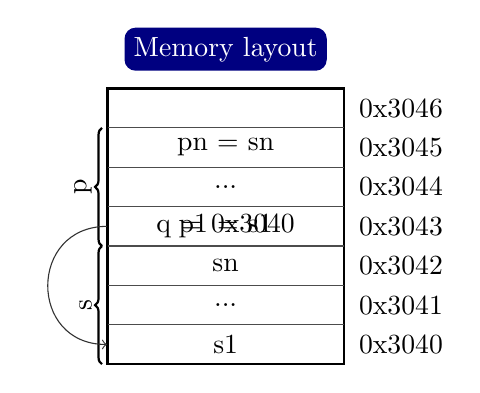
\begin{tikzpicture}
      \memorystack[word size=1, nb blocks=7, size x=3cm]
      \onslide<2-> {
        \memorypush{s1}
        \memorypush{...}
        \memorypush{sn}
        \memorystruct{1}{3}{s}
      }
      \onslide<3> {
        \memorypush{p1 = s1}
        \memorypush{...}
        \memorypush{pn = sn}
        \memorystruct{4}{6}{p}
      }
      \memorygoto{4}
      \onslide<4> {
        \memorypushpointer[q =]{1}
      }
    \end{tikzpicture}
    \vfill \null
  \end{multicols}
\end{frame}

\Scontents*[store-cmd=code_smallStruct]{
struct SmallStruct {int a;};
SmallStruct s = {1};

void changeSS(SmallStruct p) {
  p.a = 2;
}
changeSS(s);
// s.a == 1

void changeSS2(SmallStruct &q) {
  q.a = 2;
}
changeSS2(s);
// s.a == 2
}
\begin{frame}[fragile]
  \frametitlecpp[98]{Functions: pass by value or reference?}
  \begin{multicols}{2}
    \begin{overprint}[\columnwidth]
      \onslide<1>
      \highlightCppCode{}{code_smallStruct}
      \onslide<2>
      \highlightCppCode{2}{code_smallStruct}
      \onslide<3>
      \highlightCppCode{4,7}{code_smallStruct}
      \onslide<4>
      \highlightCppCode{5}{code_smallStruct}
      \onslide<5>
      \highlightCppCode{8}{code_smallStruct}
      \onslide<6>
      \highlightCppCode{10,13}{code_smallStruct}
      \onslide<7>
      \highlightCppCode{11}{code_smallStruct}
      \onslide<8>
      \highlightCppCode{14}{code_smallStruct}
    \end{overprint}
    \columnbreak
    \null \vfill
    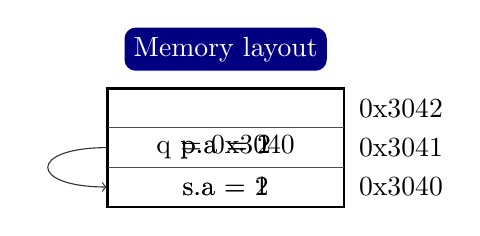
\begin{tikzpicture}
      \memorystack[word size=1, nb blocks=3, size x=3cm]
      \onslide<2-6> {
        \memorypush{s.a = 1}
      }
      \memorygoto{1}
      \onslide<7-> {
        \memorypush{s.a = 2}
      }

      \memorygoto{2}
      \onslide<3> {
        \memorypush{p.a = 1}
      }
      \memorygoto{2}
      \onslide<4> {
        \memorypush{p.a = 2}
      }
      \memorygoto{2}
      \onslide<6-7> {
        \memorypushpointer[q =]{1}
      }
      \end{tikzpicture}
    \vfill \null
  \end{multicols}
\end{frame}

\begin{frame}[fragile]
  \frametitlecpp[98]{Pass by value, reference or pointer}
  \begin{block}{Different ways to pass arguments to a function}
    \begin{itemize}
    \item by default, arguments are passed by value (= copy) \\
          good for small types, e.g.\ numbers
    \item prefer references for mandatory parameters to avoid copies
    \item use pointers for optional parameters to allow \mintinline{cpp}{nullptr}
    \item use \mintinline{cpp}{const} for safety and readability whenever possible
    \end{itemize}
  \end{block}
  \pause
  \begin{block}{Syntax}
    \begin{cppcode*}{escapeinside=||}
struct T {...}; T a;
void f(T value);           f(a);      // by value
void fRef(const T &value); fRef(a);   // by reference
void fPtr(const T *value); fPtr(|{\setlength{\fboxsep}{0pt}\color{gray}\colorbox{yellow}{\textsc{&}}}|a);  // by pointer
void fWrite(T &value);     fWrite(a); // non-const ref
    \end{cppcode*}
  \end{block}
\end{frame}

\begin{frame}[fragile]
  \frametitlecpp[98]{Functions}
  \begin{alertblock}{Exercise}
    Familiarise yourself with pass by value / pass by reference.
    \begin{itemize}
      \item go to \texttt{code/functions}
      \item Look at \texttt{functions.cpp}
      \item Compile it (\texttt{make}) and run the program (\texttt{./functions})
      \item Work on the tasks that you find in \texttt{functions.cpp}
    \end{itemize}
  \end{alertblock}
\end{frame}

\begin{frame}[fragile]
  \frametitlecpp[98]{Functions: good practices}
  \begin{onlyenv}<1>
    \begin{block}{Ensure good readability/maintainability:}
      \begin{itemize}
        \item Keep functions short
        \item Do one logical thing (single-responsibility principle)
        \item Use expressive names
        \item Document non-trivial functions
      \end{itemize}
    \end{block}
    \begin{exampleblock}{Example: Good}
      \begin{cppcode*}{gobble=2}
        /// Count number of dilepton events in data.
        /// \param d Dataset to search.
        unsigned int countDileptons(Data d) {
          selectEventsWithMuons(d);
          selectEventsWithElectrons(d);
          return d.size();
        }
      \end{cppcode*}
    \end{exampleblock}
  \end{onlyenv}
  \begin{onlyenv}<2->
    \begin{alertblock}{Example: don't! Everything in one long function}
      \begin{multicols}{2}
        \begin{cppcode*}{gobble=6}
          unsigned int runJob() {
            // Step 1: data
            Data data;
            data.resize(123456);
            data.fill(...);

            // Step 2: muons
            for (....) {
              if (...) {
                data.erase(...);
              }
            }
            // Step 3: electrons
            for (....) {
        \end{cppcode*}
        \columnbreak
        \begin{cppcode*}{gobble=6,firstnumber=last}
              if (...) {
                data.erase(...);
              }
            }

            // Step 4: dileptons
            int counter = 0;
            for (....) {
              if (...) {
                counter++;
              }
            }

            return counter;
          }
        \end{cppcode*}
      \end{multicols}
    \end{alertblock}
  \end{onlyenv}
\end{frame}

\subsection[Op]{Operators}

\begin{frame}[fragile]
  \frametitlecpp[98]{Operators(1)}
  \begin{block}{Binary and Assignment Operators}
    \begin{cppcode*}{}
      int i = 1 + 4 - 2;  // 3
      i *= 3;             // 9, short for: i = i * 3;
      i /= 2;             // 4
      i = 23 % i;         // modulo => 3
    \end{cppcode*}
  \end{block}
  \pause
  \begin{block}{Increment / Decrement Operators \uncover<3->{\hfill \alert{\bf Use wisely}}}
    \begin{cppcode*}{}
      int i = 0; i++; // i = 1
      int j = ++i;    // i = 2, j = 2
      int k = i++;    // i = 3, k = 2
      int l = --i;    // i = 2, l = 2
      int m = i--;    // i = 1, m = 2
    \end{cppcode*}
  \end{block}
\end{frame}

\begin{frame}[fragile]
  \frametitlecpp[98]{Operators(2)}
  \begin{block}{Bitwise and Assignment Operators}
    \begin{cppcode*}{}
      unsigned i = 0xee & 0x55;  // 0x44
      i |= 0xee;                 // 0xee
      i ^= 0x55;                 // 0xbb
      unsigned j = ~0xee;        // 0xffffff11
      unsigned k = 0x1f << 3;    // 0xf8
      unsigned l = 0x1f >> 2;    // 0x7
    \end{cppcode*}
  \end{block}
  \pause
  \begin{block}{Logical Operators}
    \begin{cppcode*}{}
      bool a = true;
      bool b = false;
      bool c = a && b;    // false
      bool d = a || b;    // true
      bool e = !d;        // false
    \end{cppcode*}
  \end{block}
\end{frame}

\begin{frame}[fragile]
  \frametitlecpp[98]{Operators(3)}
  \begin{block}{Comparison Operators}
    \begin{cppcode*}{}
      bool a = (3 == 3);  // true
      bool b = (3 != 3);  // false
      bool c = (4 <  4);  // false
      bool d = (4 <= 4);  // true
      bool e = (4 >  4);  // false
      bool f = (4 >= 4);  // true
      auto g = (5 <=> 5); // C++20 (later)
    \end{cppcode*}
  \end{block}
  \pause
  \begin{block}{Precedences \uncover<3->{\hfill \alert{\bf Avoid}\uncover<4->{\color{green} \bf\ - use parentheses}}}
    \begin{cppcode*}{linenos=false}
      c &= 1+(++b)|(a--)*4%5^7; // ???
    \end{cppcode*}
    Details can be found on {\color{blue!50!white} \href{https://en.cppreference.com/w/cpp/language/operator_precedence}{cppreference}}
  \end{block}
\end{frame}

\subsection[Control]{Control structures}

\begin{frame}[fragile]
  \frametitlecpp[98]{Control structures: if}
  \begin{block}{if syntax}
    \begin{cppcode*}{}
      if (condition1) {
        Statement1; Statement2;
      } else if (condition2)
        OnlyOneStatement;
      else {
        Statement3;
        Statement4;
      }
    \end{cppcode*}
    \begin{itemize}
      \item The \mintinline{cpp}{else} and \mintinline{cpp}{else if} clauses are optional
      \item The \mintinline{cpp}{else if} clause can be repeated
      \item Braces are optional if there is a single statement
    \end{itemize}
  \end{block}
\end{frame}

\begin{frame}[fragile]
  \frametitlecpp[98]{Control structures: if}
  \begin{exampleblock}{Practical example}
    \begin{cppcode*}{}
      int collatz(int a) {
        if (a <= 0) {
          std::cout << "not supported";
          return 0;
        } else if (a == 1) {
          return 1;
        } else if (a%2 == 0) {
          return collatz(a/2);
        } else {
          return collatz(3*a+1);
        }
      }
    \end{cppcode*}
  \end{exampleblock}
\end{frame}

\begin{frame}[fragile]
  \frametitlecpp[98]{Control structures: conditional operator}
  \begin{block}{Syntax}
    \begin{cppcode*}{linenos=false}
      test ? expression1 : expression2;
    \end{cppcode*}
    \vspace{-0.2cm}
    \begin{itemize}
      \item If test is \mintinline{cpp}{true} expression1 is returned
      \item Else, expression2 is returned
    \end{itemize}
  \end{block}
  \pause
  \begin{exampleblock}{Practical example}
    \begin{cppcode*}{}
      int collatz(int a) {
        return a==1 ? 1 : collatz(a%2==0 ? a/2 : 3*a+1);
      }
    \end{cppcode*}
  \end{exampleblock}
  \pause
  \begin{alertblock}{Do not abuse it}
    \begin{itemize}
      \item Explicit \mintinline{cpp}{if}s are generally easier to read
      \item Use the ternary operator with short conditions and expressions
      \item Avoid nesting
    \end{itemize}
  \end{alertblock}
\end{frame}

\begin{frame}[fragile]
  \frametitlecpp[98]{Control structures: switch}
  \begin{block}{Syntax}
    \begin{cppcode*}{gobble=2}
      switch(identifier) {
        case c1 : statements1; break;
        case c2 : statements2; break;
        case c3 : statements3; break;
        ...
        default : instructiond; break;
      }
    \end{cppcode*}
    \begin{itemize}
      \item The \mintinline{cpp}{break} statement is not mandatory but...
      \item Cases are entry points, not independent pieces
      \item Execution falls through to the next case without a \mintinline{cpp}{break}!
      \item The \mintinline{cpp}{default} case may be omitted
    \end{itemize}
  \end{block}
  \pause
  \begin{alertblock}{Use break}
    Avoid \mintinline{cpp}{switch} statements with fall-through cases
  \end{alertblock}
\end{frame}

\begin{frame}[fragile]
  \frametitlecpp[98]{Control structures: switch}
  \begin{exampleblock}{Practical example}
    \begin{cppcode*}{}
      enum class Lang { French, German, English, Other };
      ...
      switch (language) {
      case Lang::French:
        std::cout << "Bonjour";
        break;
       case Lang::German:
        std::cout << "Guten Tag";
        break;
      case Lang::English:
        std::cout << "Good morning";
        break;
      default:
        std::cout << "I do not speak your language";
      }
    \end{cppcode*}
  \end{exampleblock}
\end{frame}

\AtBeginEnvironment{minted}{\renewcommand{\fcolorbox}[4][]{#4}}

\begin{frame}[fragile]
  \frametitlecpp[17]{\texttt{[[fallthrough]]} attribute}
  \begin{block}{New compiler warning}
    Since \cpp17, compilers are encouraged to warn on fall-through
  \end{block}
  \begin{exampleblock}{\cpp17}
    \begin{cppcode*}{}
      switch (c) {
        case 'a':
          f();    // Warning emitted
        case 'b': // Warning emitted
        case 'c':
          g();
          [[fallthrough]]; // Warning suppressed
        case 'd':
          h();
      }
    \end{cppcode*}
  \end{exampleblock}
\end{frame}

\begin{frame}[fragile]
  \frametitlecpp[17]{Init-statements for if and switch}
  \begin{block}{}
    Allows to limit variable scope in \mintinline{cpp}{if} and \mintinline{cpp}{switch} statements
  \end{block}
  \begin{exampleblock}{\cpp17}
    \begin{cppcode*}{}
      if (Value val = GetValue(); condition(val)) {
        f(val);
      } else {
        g(val);
      }
      h(val); // compile error
    \end{cppcode*}
  \end{exampleblock}
  \pause
  \begin{alertblock}{\cpp98}
    Don't confuse with a variable declaration as condition:
    \begin{cppcode*}{firstnumber=7}
      if (Value* val = GetValuePtr())
        f(*val);
    \end{cppcode*}
  \end{alertblock}
\end{frame}

\begin{frame}[fragile]
  \frametitlecpp[98]{Control structures: for loop}
  \begin{block}{for loop syntax}
    \begin{cppcode*}{}
      for(initializations; condition; increments) {
        statements;
      }
    \end{cppcode*}
    \vspace{-0.2cm}
    \begin{itemize}
      \item Initializations and increments are comma separated
      \item Initializations can contain declarations
      \item Braces are optional if loop body is a single statement
    \end{itemize}
  \end{block}
  \pause
  \begin{exampleblock}{Practical example}
    \begin{cppcode*}{firstnumber=4}
      for(int i = 0, j = 0 ; i < 10 ; i++, j = i*i) {
        std::cout << i << "^2 is " << j << '\n';
      }
    \end{cppcode*}
  \end{exampleblock}
  \pause
  \begin{goodpracticeWithShortcut}{Don't abuse the \texttt{for} syntax}{\texttt{for} syntax}
    \begin{itemize}
      \item The \mintinline{cpp}{for} loop head should fit in 1-3 lines
    \end{itemize}
  \end{goodpracticeWithShortcut}
\end{frame}

\begin{frame}[fragile]
  \frametitlecpp[11]{Range-based loops}
  \begin{block}{Reason of being}
    \begin{itemize}
    \item Simplifies loops over ``ranges'' tremendously
    \item Especially with STL containers
    \end{itemize}
  \end{block}
  \begin{block}{Syntax}
    \begin{cppcode*}{}
      for ( type iteration_variable : range ) {
        // body using iteration_variable
      }
    \end{cppcode*}
  \end{block}
  \begin{exampleblock}{Example code}
    \begin{cppcode*}{firstnumber=4}
      int v[4] = {1,2,3,4};
      int sum = 0;
      for (int a : v) { sum += a; }
    \end{cppcode*}
  \end{exampleblock}
\end{frame}

\begin{frame}[fragile]
  \frametitlecpp[20]{Init-statements for range-based loops}
  \begin{block}{}
    Allows to limit variable scope in range-based loops
  \end{block}
  \begin{alertblock}{\cpp17}
    \begin{cppcode*}{}
      std::array data = {"hello", ",", "world"};
      std::size_t i = 0;
      for (auto& d : data) {
        std::cout << i++ << ' ' << d << '\n';
      }
    \end{cppcode*}
  \end{alertblock}
  \begin{exampleblock}{\cpp20}
    \begin{cppcode*}{firstnumber=6}
      std::array data = {"hello", ",", "world"};
      for (std::size_t i = 0; auto& d : data) {
        std::cout << i++ << ' ' << d << '\n';
      }
    \end{cppcode*}
  \end{exampleblock}
\end{frame}

\begin{frame}[fragile]
  \frametitlecpp[98]{Control structures: while loop}
  \begin{block}{while loop syntax}
    \begin{cppcode*}{}
      while(condition) {
        statements;
      }
      do {
        statements;
      } while(condition);
    \end{cppcode*}
    \begin{itemize}
      \item Braces are optional if the body is a single statement
    \end{itemize}
  \end{block}
  \pause
  \begin{alertblock}{Bad example}
    \begin{cppcode*}{}
      while (n != 1)
        if (0 == n%2) n /= 2;
        else n = 3 * n + 1;
    \end{cppcode*}
  \end{alertblock}
\end{frame}

\begin{frame}[fragile]
  \frametitlecpp[98]{Control structures: jump statements}
  \begin{block}{}
    \begin{description}
    \item[break] Exits the loop and continues after it
    \item[continue] Goes immediately to next loop iteration
    \item[return] Exits the current function
    \item[goto] Can jump anywhere inside a function, avoid!
    \end{description}
  \end{block}
  \pause
  \begin{alertblock}{Bad example}
    \begin{cppcode*}{}
      while (1) {
        if (n == 1) break;
        if (0 == n%2) {
          std::cout << n << '\n';
          n /= 2;
          continue;
        }
        n = 3 * n + 1;
      }
    \end{cppcode*}
  \end{alertblock}
\end{frame}

\begin{frame}[fragile]
  \frametitlecpp[11]{Control structures}
  \begin{exerciseWithShortcut}{Control structures}{Control structs}
    Familiarise yourself with different kinds of control structures. Re-implement them in different ways.
    \begin{itemize}
      \item Go to \texttt{code/control}
      \item Look at \texttt{control.cpp}
      \item Compile it (\texttt{make}) and run the program (\texttt{./control})
      \item Work on the tasks that you find in \texttt{README.md}
    \end{itemize}
  \end{exerciseWithShortcut}
\end{frame}

\subsection[.h]{Headers and interfaces}

\begin{frame}[fragile]
  \frametitlecpp[98]{Headers and interfaces}
  \begin{block}{Interface}
    Set of declarations defining some functionality
    \begin{itemize}
    \item Put in a so-called ``header file''
    \item The implementation exists somewhere else
    \end{itemize}
  \end{block}
  \begin{block}{Header: hello.hpp}
    \begin{cppcode*}{linenos=false}
      void printHello();
    \end{cppcode*}
  \end{block}
  \begin{block}{Usage: myfile.cpp}
    \begin{cppcode*}{}
      #include "hello.hpp"
      int main() {
        printHello();
      }
    \end{cppcode*}
  \end{block}
\end{frame}

\begin{frame}[fragile]
  \frametitlecpp[98]{Preprocessor}
  \begin{cppcode}
    // file inclusion
    #include "hello.hpp"
    // macro constants and function-style macros
    #define MY_GOLDEN_NUMBER 1746
    #define CHECK_GOLDEN(x) if ((x) != MY_GOLDEN_NUMBER) \
      std::cerr << #x " was not the golden number\n";
    // compile time or platform specific configuration
    #if defined(USE64BITS) || defined(__GNUG__)
      using myint = std::uint64_t;
    #elif
      using myint = std::uint32_t;
    #endif
  \end{cppcode}
  \pause
  \begin{goodpracticeWithShortcut}{Use preprocessor only in very restricted cases}{preprocessor}
    \begin{itemize}
      \item Conditional inclusion of headers
      \item Customization for specific compilers/platforms
    \end{itemize}
  \end{goodpracticeWithShortcut}
\end{frame}

\begin{frame}[fragile]
  \frametitlecpp[98]{Header include guards}
  \begin{block}{Problem: redefinition by accident}
    \begin{itemize}
      \item Headers may define new names (e.g.\ types)
      \item Multiple (transitive) inclusions of a header would define those names multiple times, which is a compile error
      \item Solution: guard the content of your headers!
    \end{itemize}
  \end{block}
  \begin{block}{Include guards}
    \begin{cppcode*}{}
      #ifndef MY_HEADER_INCLUDED
      #define MY_HEADER_INCLUDED
      ... // header file content
      #endif
    \end{cppcode*}
  \end{block}
  \begin{block}{Pragma once (non-standard)}
    \begin{cppcode*}{}
      #pragma once
      ... // header file content
    \end{cppcode*}
  \end{block}
\end{frame}

\subsection[auto]{Auto keyword}

\begin{frame}[fragile]
  \frametitlecpp[11]{Auto keyword}
  \begin{block}{Reason of being}
    \begin{itemize}
    \item Many type declarations are redundant
    \item They are often a source for compiler warnings and errors
    \item Using auto prevents unwanted/unnecessary type conversions
    \end{itemize}
    \begin{cppcode*}{}
      std::vector<int> v;
      float a = v[3];    // conversion intended?
      int b = v.size();  // bug? unsigned to signed
    \end{cppcode*}
  \end{block}
  \pause
  \begin{block}{Practical usage}
    \begin{cppcode*}{}
      std::vector<int> v;
      auto a = v[3];
      const auto b = v.size(); // std::size_t
      int sum{0};
      for (auto n : v) { sum += n; }
    \end{cppcode*}
  \end{block}
\end{frame}

\begin{frame}[fragile]
  \frametitlecpp[98]{Loops, references, auto}
  \begin{exerciseWithShortcut}{Loops, references, auto}{Loops, refs, auto}
    Familiarise yourself with range-based for loops and references
    \begin{itemize}
      \item Go to \texttt{exercises/loopsRefsAuto}
      \item Look at \texttt{loopsRefsAuto.cpp}
      \item Compile it (\texttt{make}) and run the program (\texttt{./loopsRefsAuto})
      \item Work on the tasks that you find in \texttt{loopsRefsAuto.cpp}
    \end{itemize}
  \end{exerciseWithShortcut}
\end{frame}



\section[OO]{Object orientation}
%%\includeonlyframes{current}

\subsection{Objects and Classes}

\begin{frame}[fragile]
  \frametitle{What are classes and objects}
  \begin{block}{Classes}
    structs on steroids
    \begin{itemize}
    \item with inheritance
    \item with associated methods
    \end{itemize}
  \end{block}
  \begin{block}{Objects}
    instances of classes
  \end{block}
  \begin{block}{Encapsulates a concept}
    \begin{itemize}
    \item shows an interface
    \item provides its implementation
      \begin{itemize}
      \item status, properties
      \item possible interactions
      \item construction and destruction
      \end{itemize}    
    \end{itemize}    
  \end{block}
\end{frame}


\begin{frame}[fragile]
  \frametitle{My First Class}
  \begin{multicols}{2}
    \begin{cppcode*}{gobble=6}
      struct MyFirstClass {
        int a;
        void squareA() {
          a *= a;
        };
      };

      MyFirstClass myObj;
      myObj.a = 2;

      // let's square a
      myObj.squareA();
    \end{cppcode*}
    \columnbreak
    \null \vfill
    \begin{tikzpicture}
      \tcbset{minted options={gobble=8}}
      \begin{CodeNode}{0,-2}{MyFirstClass}{MyFirstClass}
        int a;
        void squareA();
      \end{CodeNode}
    \end{tikzpicture}
    \vfill \null
  \end{multicols}
\end{frame}




\begin{frame}[fragile,label=current]
\xxx
  \frametitle{Static members}
  \begin{block}{Concept}
    \begin{itemize}
    \item members attached to a class rather than to an object
    \item usable with or without an instance of the class
    \item identified by the {\it static} keyword
    \end{itemize}
  \end{block}
  \begin{cppcode*}{}
    Class Text {
    public:
      static std::string upper(std::string);
    private:
      static int s_bCallsToUpper;
    }
    int Text::s_bCallsToUpper = 0;
    std::string s = "my text";
    std::string uppers = Text::upper("my text");
    // now Text::s_bCallsToUpper is 1
  \end{cppcode*}
\end{frame}

\begin{frame}[fragile,label=current]
  \frametitle{private/ public inheritance}
  /xxx
\end{frame}

\begin{frame}[fragile,label=current]
  \frametitle{static functions}
  /xxx
\end{frame}

\begin{frame}[fragile,label=current]
  \frametitle{static variable}
  /xxx
\end{frame}

\begin{frame}[fragile]
  \frametitle{Separating the interface}
  \begin{block}{Header : MyFirstClass.hpp}
    \begin{cppcode*}{linenos=false,gobble=6}
      struct MyFirstClass {
        int a;
        void squareA();
      };
    \end{cppcode*}
  \end{block}
  \begin{block}{Implementation : MyFirstClass.cpp}
    \begin{cppcode*}{linenos=false,gobble=6}
      #include "MyFirstClass.hpp"
      void MyFirstClass::squareA() {
        a *= a;
      };
    \end{cppcode*}
  \end{block}
\end{frame}

\begin{frame}[fragile]
  \frametitle{A word on namespaces}
  \begin{itemize}
  \item Namespaces allow to segment your code to avoid name clashes
  \item They can be embedded to create hierarchies (separator is '::')
  \end{itemize}
  \begin{multicols}{2}
    \begin{cppcode*}{gobble=6}
      namespace n {
        int a;
      }      
      namespace p {
        int a; // no clash
        namespace inner {
          int a; // no clash
        }
      }
      int f() {
        n::a = 2;
      }
    \end{cppcode*}
    \columnbreak
    \begin{cppcode*}{gobble=6,firstnumber=13}
      namespace p {
        int f() {
          p::a = 2;
          a = 2;  //same as above
          p::inner::a = 4;
          inner::a = 4;
          n::a = 5;
        }
      }
      using namespace p::inner;
      int g() {
        a = 3; // using p::inner
      }
  \end{cppcode*}
  \end{multicols}
\end{frame}

\begin{frame}[fragile]
  \frametitle{Implementing methods}
  \begin{block}{Standard practice}
    \begin{itemize}
    \item usually in .cpp, outside of class declaration
    \item using the class name as namespace
    \item when reference to the object is needed, use {\it this} keyword
    \end{itemize}
  \end{block}
  \begin{cppcode*}{}
    void MyFirstClass::squareA() {
      a *= a;
    };

    int MySecondClass::sum() {
      int a = 0; // do not do that !
      a += this->a;
      a += this->b;
      return a;
    };
  \end{cppcode*}
\end{frame}

\begin{frame}[fragile]
  \frametitle{Method overloading}
  \begin{block}{The rules in \cpp}
    \begin{itemize}
    \item overloading is authorized and welcome
    \item signature is part of the method identity
    \item but not the return code
    \end{itemize}
  \end{block}
  \begin{cppcode*}{}
    class MySecondClass : MyFirstClass {
    public:
      int sum();
      int sum(int c);
    }

    int MySecondClass::sum() { return a + b; };

    int MySecondClass::sum(int c) { return a + b + c; };
  \end{cppcode*}
\end{frame}

\subsection{Inheritance}

\begin{frame}[fragile]
  \frametitle{First inheritance}
  \begin{multicols}{2}
    \begin{cppcode*}{gobble=6,firstnumber=13}
      struct MySecondClass :
        MyFirstClass {
        int b;
        int sum() {
          return a + b;
        };
      };

      MySecondClass myObj2;
      myObj2.a = 2;
      myObj2.b = 5;

      myObj2.squareA();
      int i = myObj2.sum();
      // i = 9
    \end{cppcode*}
    \columnbreak
    \null \vfill
    \begin{tikzpicture}
      \tcbset{minted options={gobble=8}}
      \begin{CodeNode}{0,1.5}{MyFirstClass}
        int a;
        void squareA();
      \end{CodeNode}
      \begin{CodeNode}{0,-1.5}{MySecondClass}
        int b;
        int sum();
      \end{CodeNode}
    \draw[very thick,->] (MySecondClass)--(MyFirstClass);
    \end{tikzpicture}
    \vfill \null
  \end{multicols}
\end{frame}


\subsection{Encapsulation}

\begin{frame}[fragile]
  \frametitle{Managing access to class members}
  \begin{block}{{\it public} / {\it private} keywords}
    \begin{itemize}
      \item {\it private} : access only inside the class
      \item {\it public} : access from anywhere
      \item Default is {\it private}
      \item A {\it struct} is a {\it class} fully public
    \end{itemize}
  \end{block}
  \pause
  \begin{multicols}{2}
    \begin{cppcode*}{gobble=6}
      class MyFirstClass {
      public:
        void setA(int a);
        int getA();
        void squareA();
      private:
        int a;
      }
    \end{cppcode*}
    \columnbreak
    \begin{cppcode*}{gobble=6,firstnumber=9}
      MyFirstClass obj;
      obj.a = 5;   // error !
      obj.setA(5); // ok
      obj.squareA();
      int b = obj.getA();
    \end{cppcode*}
    \pause
    \begin{tcolorbox}[left=0mm,right=0mm,top=0mm,bottom=0mm,colback=red!5!white,colframe=red!75!black]
      This breaks MySecondClass !
    \end{tcolorbox}
  \end{multicols}
\end{frame}

\begin{frame}[fragile]
  \frametitle{Managing access to class members(2)}
  \begin{block}{Solution is {\it protected} keyword}
    Gives access to class descendant
  \end{block}
  \begin{multicols}{2}
    \begin{cppcode*}{gobble=6}
      class MyFirstClass {
      public:
        void setA(int a);
        int getA();
        void squareA();
      protected:
        int a;
      }
    \end{cppcode*}
    \columnbreak
    \begin{cppcode*}{gobble=6,firstnumber=13}
      class MySecondClass :
        MyFirstClass {
      public:
        int sum() {
          return a + b;
        };
      private:
        int b;
      }
    \end{cppcode*}
  \end{multicols}
\end{frame}


\subsection{constructors and destructors}


\begin{frame}[fragile]
  \frametitle{Class Constructors and Destructor}
  \begin{block}{Concept}
    \begin{itemize}
    \item special functions building/destroying an object
    \item a class can have several constructors
    \item the constructors have the name of the class
    \item same for the destructor with a leading $\sim$
    \end{itemize}
  \end{block}
  \begin{multicols}{2}
    \begin{cppcode*}{gobble=6}
      class MyFirstClass {
      public:
        MyFirstClass();
        MyFirstClass(int a);
        ~MyFirstClass();
        ...
      protected:
        int a;
      };
    \end{cppcode*}
    \columnbreak
    \begin{cppcode*}{gobble=6,firstnumber=10}
      // note special notation for
      // initialization of members
      MyFirstClass() : a(0) {}
      
      MyFirstClass(int a_):a(_a) {}

      ~MyFirstClass(){};
    \end{cppcode*}
  \end{multicols}
\end{frame}


\begin{frame}[fragile]
  \frametitle{Class Constructor and Destructors}
  \begin{cppcode*}{}
    class Vector {
    public:
      Vector(int n);
      ~Vector();
      void setN(int n, int value);
      int getN(int n);
    private:
      int len;
      int* data;
    }
    Vector::Vector(int n) : len(n) {
      data = (int*)malloc(n*sizeof(int));
    }
    Vector::~Vector() {
      free(data);
    }
  \end{cppcode*}
\end{frame}


\begin{frame}[fragile]
  \frametitle{Constructor and inheritance}
  \begin{cppcode*}{}
    struct MyFirstClass {
      MyFirstClass();
      MyFirstClass(int a);
    }

    struct MySecondClass : MyFirstClass {
      MySecondClass();
      MySecondClass(int b);
      MySecondClass(int a, int b);
    }

    MySecondClass() : MyFirstClass(), b(0) {};
    MySecondClass(int b_) : MyFirstClass(), b(b_) {};
    MySecondClass(int a_,
                  int b_) : MyFirstClass(a_), b(b_) {};
  \end{cppcode*}
\end{frame}

\begin{frame}[fragile]
  \frametitle{Object lifetime}
  \begin{block}{On the stack}
    \begin{itemize}
    \item object are created when declared (constructor called)
    \item object are destructed when out of scope (destructor is called)
    \end{itemize}
  \end{block}
  \begin{cppcode*}{}
    {
      MyFirstClass a; // default constructor called
      ...
    }  // destructor called

    int f() {
      MyFirstClass a(3); // constructor called
      ...
    } // destructor called
  \end{cppcode*}
\end{frame}

\begin{frame}[fragile]
  \frametitle{Object lifetime}
  \begin{block}{On the heap}
    \begin{itemize}
    \item object are created by calling {\it new} (constructor is called)
    \item object are destructed by calling {\it delete} (destructor is called)
    \end{itemize}
  \end{block}
  \begin{cppcode*}{}
    {
      // default constructor called
      MyFirstClass *a = new MyFirstClass;
      ...
      delete a; // destructor is called
    }

    int f() {
      // constructor called
      MyFirstClass *a = new MyFirstClass(3);
      ...
    } // memory leak !!!
  \end{cppcode*}
\end{frame}

\subsection{Exceptions}

\begin{frame}[fragile]
  \frametitle{Exceptions}
  \begin{block}{The concept}
    \begin{itemize}
    \item exceptional Event breaking linearity of the code
    \item will be handled in dedicated place
    \end{itemize}
  \end{block}
  \begin{block}{Pratically}
    \begin{itemize}
    \item you can throw any object with {\it throw}
    \item you handle them using {\it try ... catch} blocks
    \end{itemize}
  \end{block}
  \begin{cppcode*}{}
    try {
      if (0 == name) {
        throw std::string("Expected non empty name");
      }
      printf("%s\n", name);
    } catch (std::string e) {
      printf("empty name found\n");      
    }
  \end{cppcode*}
\end{frame}

\begin{frame}[fragile]
  \frametitle{Exceptions}
  \begin{block}{Rules}
    \begin{itemize}
    \item exception will skip all code until next {\it catch}
    \begin{itemize}
      \item still destructors are called when exiting scopes
      \item but your own cleanup may not be
    \end{itemize}
    \item {\it catch} is selective on the exception type
    \end{itemize}
  \end{block}
  \begin{multicols}{2}
    \begin{cppcode*}{fontsize=\scriptsize,gobble=6}
      class ZeroDivide {};
      
      int divide(int a, int b) {
        if (0 == b) {
          throw ZeroDivide();
        }
        return a/b;
      }
    \end{cppcode*}
    \columnbreak
    \begin{cppcode*}{fontsize=\scriptsize,gobble=6,firstnumber=9} 
      int func(char* value) {
        try {
          errno = 0;
          long l = strtol(value,0,10);
          if (errno) {
            throw string("Bad Value");
          }
          divide(100, l);
        } catch (string e) {
          printf("%s\n", e.c_str());
        } catch (ZeroDivide e2) {
          printf("Division error\n");
        }
      }
    \end{cppcode*}
  \end{multicols}
\end{frame}

\xxx throw declaration for a function
\xxx only at run time !!!


\section{Advanced Topics}

\subsection[Functions]{More around functions}
\subsubsection{Functors}
\subsubsection{Pointers and references}
\subsubsection{Constness}

\subsection[Inheritance]{Advanced inheritance}
\subsubsection{Statics}
\subsubsection{Virtual members}
\subsubsection{Virtual inheritance}

\subsection{Templates}
\subsubsection[Functions]{Templated functions}
\subsubsection[Classes]{Templated classes}

\subsection[STL]{The Standard Template Library}
\subsubsection[Containers]{Standard containers}
\subsubsection[Customization]{Allocators. comparators and other containers}
\subsubsection{Algorithms}

\subsection[Tools]{Useful tools}
\subsubsection{Compilers}
\subsubsection{Static analyzer}
\subsubsection{Debugger}
\subsubsection{Memory checker}



%\section[C$^{++}$11]{C$^{++}$11 preview}
\subsection[Auto]{auto keyword}
\subsection{Easy loops}
\subsection{Lambdas}
\subsection{Move semantic}
\subsection{Smart pointers}


\end{document}
